% Tabela: Resultados do Experimento Omega
\begin{figure*}[hb]
	\centering
		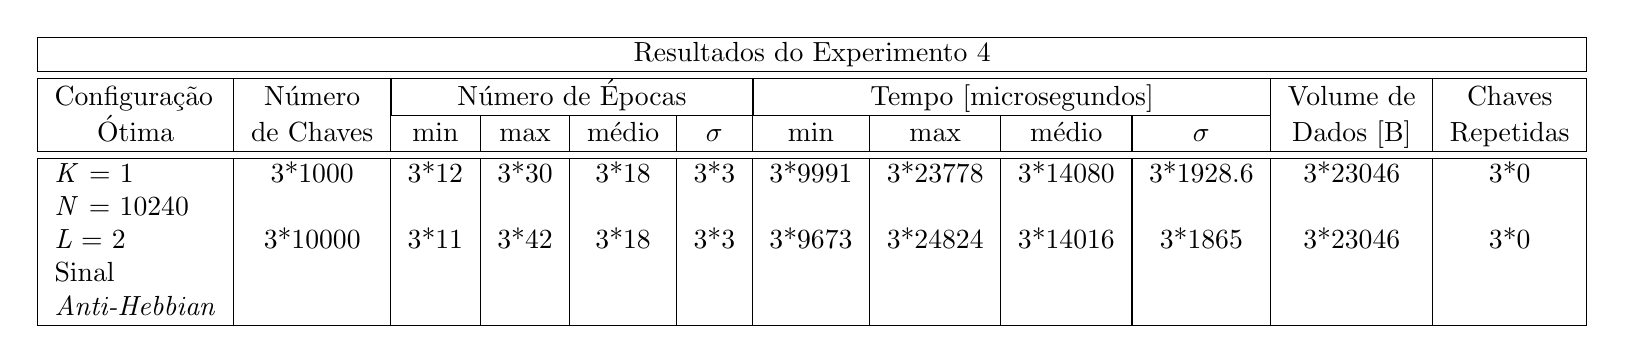
\begin{tikzpicture}
			
		\node[thick, align=center] (table) {
			\begin{tabular}{ |l|c|c|c|c|c|c|c|c|c|c|c| }
				\hline
				\multicolumn{12}{ |c| }{Resultados do Experimento 4} \\
				\hline \hline
				Configuração &
				Número &
				\multicolumn{4}{ |c| }{Número de Épocas} &
				\multicolumn{4}{ |c| }{Tempo [microsegundos]} &
				Volume de &
				Chaves\\ \cline{3-10}

				\multicolumn{1}{|c|}{Ótima} & de Chaves & min & max & médio & $\sigma$ & min & max & médio & $\sigma$ & Dados [B] & Repetidas\\
				\hline \hline
				
				\textit{K} = 1 &
				\multirow{3}{*}{1000} &
				\multirow{3}{*}{12} &
				\multirow{3}{*}{30} &
				\multirow{3}{*}{18} &
				\multirow{3}{*}{3} &
				\multirow{3}{*}{9991} &
				\multirow{3}{*}{23778} &
				\multirow{3}{*}{14080} &
				\multirow{3}{*}{1928.6} &
				\multirow{3}{*}{23046} &
				\multirow{3}{*}{0} \\
				
				\textit{N} = 10240 & & & & & & & & & & &\\
				
				\textit{L} = 2 &
				\multirow{3}{*}{10000} &
				\multirow{3}{*}{11} &
				\multirow{3}{*}{42} &
				\multirow{3}{*}{18} &
				\multirow{3}{*}{3} &
				\multirow{3}{*}{9673} &
				\multirow{3}{*}{24824} &
				\multirow{3}{*}{14016} &
				\multirow{3}{*}{1865} &
				\multirow{3}{*}{23046} &
				\multirow{3}{*}{0} \\
				
				
				Sinal & & & & & & & & & & &\\
				\textit{Anti-Hebbian} & & & & & & & & & & &\\
				
				\hline
			\end{tabular}
		};

		\end{tikzpicture}
	\caption{Tabela de resultados do Experimento 4.}
	\label{tab:resultsOmega}
\end{figure*}